
\documentclass{beamer}
\usepackage[utf8]{inputenc}

\usetheme{Madrid}
\usecolortheme{default}
\usepackage{amsmath,amssymb,amsfonts,amsthm}
\usepackage{txfonts}
\usepackage{tkz-euclide}
\usepackage{listings}
\usepackage{adjustbox}
\usepackage{array}
\usepackage{tabularx}
\usepackage{gvv}
\usepackage{lmodern}
\usepackage{circuitikz}
\usepackage{tikz}
\usepackage{graphicx}

\setbeamertemplate{page number in head/foot}[totalframenumber]

\usepackage{tcolorbox}
\tcbuselibrary{minted,breakable,xparse,skins}



\definecolor{bg}{gray}{0.95}
\DeclareTCBListing{mintedbox}{O{}m!O{}}{%
  breakable=true,
  listing engine=minted,
  listing only,
  minted language=#2,
  minted style=default,
  minted options={%
    linenos,
    gobble=0,
    breaklines=true,
    breakafter=,,
    fontsize=\small,
    numbersep=8pt,
    #1},
  boxsep=0pt,
  left skip=0pt,
  right skip=0pt,
  left=25pt,
  right=0pt,
  top=3pt,
  bottom=3pt,
  arc=5pt,
  leftrule=0pt,
  rightrule=0pt,
  bottomrule=2pt,
  toprule=2pt,
  colback=bg,
  colframe=orange!70,
  enhanced,
  overlay={%
    \begin{tcbclipinterior}
    \fill[orange!20!white] (frame.south west) rectangle ([xshift=20pt]frame.north west);
    \end{tcbclipinterior}},
  #3,
}
\lstset{
    language=C,
    basicstyle=\ttfamily\small,
    keywordstyle=\color{blue},
    stringstyle=\color{orange},
    commentstyle=\color{green!60!black},
    numbers=left,
    numberstyle=\tiny\color{gray},
    breaklines=true,
    showstringspaces=false,
}
\begin{document}

\title 
{4.7.62}
\date{September 14,2025}


\author 
{EE25BTECH11065-Yoshita J}






\frame{\titlepage}
\begin{frame}{Question}
Find the equation of the plane which passes through the point (5, 2, -4) and perpendicular to the line with direction ratios 2, 3, -1.\\

\end{frame}


\begin{frame}{Theoretical Solution}
The plane passes through the point
\[
\mathbf{A} = \myvec{5\\2\\-4}
\]
with normal vector
\[
\mathbf{n} = \myvec{2\\3\\-1}.
\]

The equation of the plane can be written as
\[
\mathbf{n}^T(\mathbf{x}-\mathbf{A})=0.
\]

Equivalently,
\[
\mathbf{n}^T\mathbf{x}=\mathbf{n}^T\mathbf{A}.
\]
\end{frame}

\begin{frame}{Theoretical Solution}
Substituting the values,
\begin{align}
\myvec{2 & 3 & -1}\mathbf{x} &= \myvec{2 & 3 & -1}\myvec{5\\2\\-4} \\
\implies \myvec{2 & 3 & -1}\mathbf{x} &= 20.
\end{align}

Hence, the equation of the plane is
\[
\mathbf{n}^T\mathbf{x} = 20,
\]
where
\[
\mathbf{n} = \myvec{2\\3\\-1}.
\]

\end{frame}

\begin{frame}[fragile]
    \frametitle{C Code}

    \begin{lstlisting}
#include<stdio.h>
typedef struct {
    double x, y, z;
} Vector;

typedef struct {
    double a, b, c, d;
} Plane;

Plane find_plane_from_point_and_normal(Vector point, Vector normal) {
    Plane result;
    result.a = normal.x;
    result.b = normal.y;
    result.c = normal.z;
    result.d = (normal.x * point.x) + (normal.y * point.y) + (normal.z * point.z);
    return result;
}
    \end{lstlisting}
\end{frame}


\begin{frame}[fragile]
    \frametitle{Python Code}
    \begin{lstlisting}
import numpy as np
import matplotlib.pyplot as plt
from mpl_toolkits.mplot3d import Axes3D

point_A = np.array([5.0, 2.0, -4.0])
normal_n = np.array([2.0, 3.0, -1.0])

d = np.dot(normal_n, point_A)
plane_eq_str = f"{normal_n[0]:.0f}x + {normal_n[1]:.0f}y + {normal_n[2]:.0f}z = {d:.0f}"
print(f"Plane equation: {plane_eq_str}")

fig = plt.figure(figsize=(10, 8))
ax = fig.add_subplot(111, projection='3d')
    \end{lstlisting}
\end{frame}

\begin{frame}[fragile]
    \frametitle{Python Code}
    \begin{lstlisting}
x_range = np.linspace(point_A[0] - 5, point_A[0] + 5, 20)
y_range = np.linspace(point_A[1] - 5, point_A[1] + 5, 20)
x_grid, y_grid = np.meshgrid(x_range, y_range)

z_plane = (d - normal_n[0] * x_grid - normal_n[1] * y_grid) / normal_n[2]

ax.plot_surface(x_grid, y_grid, z_plane, alpha=0.6, cmap='plasma', edgecolor='none')

ax.scatter([point_A[0]], [point_A[1]], [point_A[2]], color='red', s=100, label=f'Point A {tuple(point_A)}')

   
    \end{lstlisting}
\end{frame}

\begin{frame}[fragile]
    \frametitle{Python Code}
    \begin{lstlisting}
ax.quiver(
    point_A[0], point_A[1], point_A[2],
    normal_n[0], normal_n[1], normal_n[2],
    length=4, normalize=True, color='black', arrow_length_ratio=0.2,
    label=f'Normal Vector n={tuple(normal_n)}'
)

ax.set_xlabel('X-axis')
ax.set_ylabel('Y-axis')
ax.set_zlabel('Z-axis')
ax.set_title(f'Plane Visualization: {plane_eq_str}', fontsize=14)
ax.legend()
plt.grid(True)
plt.show()
   
    \end{lstlisting}
\end{frame}
\begin{frame}{Plot}
    \centering
    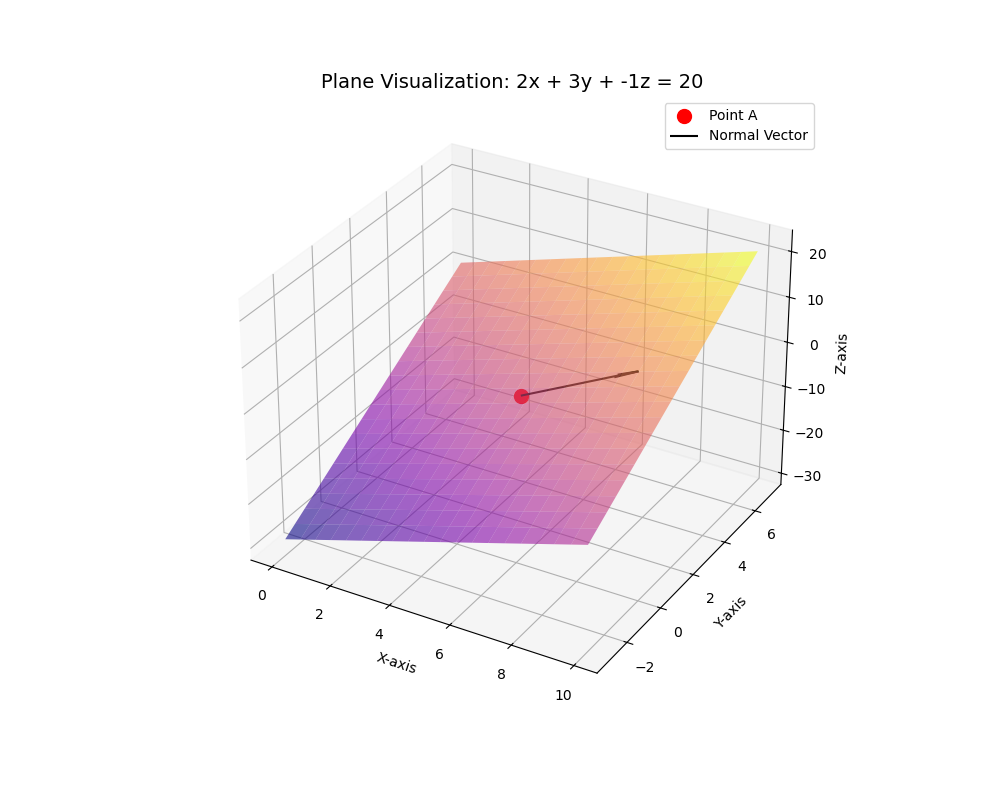
\includegraphics[width=\columnwidth, height=0.9\textheight, keepaspectratio]{figs/fig3.png}     
\end{frame}


\end{document}
